%! Author = Админ
%! Date = 18.02.2022

% Packages
\usepackage{amsmath}
\usepackage[dvipdfm]{graphicx}
\usepackage{mathtools}

\graphicspath{{pictures/}}
\DeclareGraphicsExtensions{.pdf,.png,.jpg}


% Document
\begin{document}
    \begin{center}
        \\textrm{Problem 1}
    \end{center}
    \\textrm{a).}
    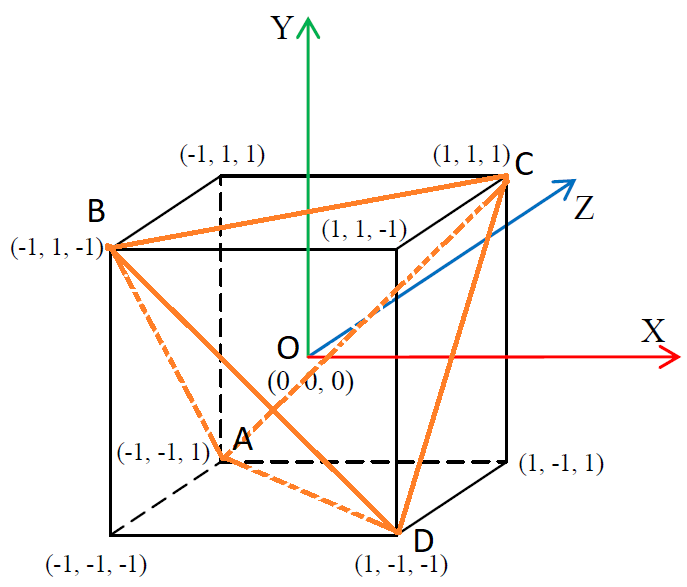
\includegraphics[width=100px]{cube}
    \(\overline{|BC|}=(c_{1})-b_{1};c_{2})-b_{2};c_{3})-b_{3})=(2;0;2)\)
    \[l=\overline{|BC|}=\sqrt{x^2 + y^2 + z^2}=2\sqrt{2}\]
    \\textrm{BC equals to the diagonal of the square, and since all faces of the cube are equal squares, so their diagonals are equal too.}
    \\textrm{b).}
    \\textrm{The angle between H and C is equal to the angle between the vectors |\overline{OB}| and |\overline{OC}| :}
    \[\angle \alpha = \arccos(\frac {\overline{OB}\cdot \overline{OC}}{|\overline{OB}| |\overline{OC}|}) = 121 \degree\]
    \\textrm{c).}
    \[\angle (CBD) = \arccos(\frac {\overline{BC}\cdot \overline{BD}}{|\overline{BC}| |\overline{BD}|}) = 60 \degree\]
    \[\angle \betta = \arccos(\frac {\overline{AB}\cdot \overline{DC}}{|\overline{AB}| |\overline{DC}|}) = 90 \degree \]
    \\textrm{d).}
    \[S = \frac{BC^2\cdot\sqrt{3}}{4} = 2\sqrt{3}\]

    \begin{center}
        \\textrm{Problem 2}
    \end{center}
    \\textrm{a).}
    \[\overline{v_1}\cdot(\overline{v_2}-\overline{v_3})=0\]
    \\textrm{b-c).}
    \[\overline{v_1}\cdot\overline{v_2}=\overline{v_1}\cdot\overline{v_3}=\overline{v_2}\cdot\overline{v_3}\]
    \[=> \overline{v_1}=\overline{v_2}=\overline{v_3}\ => \triangle\] \textrm{ is equilateral and } P \textrm{P is also on the altitude from } \[P_3\]

    \begin{center}
        \\textrm{Problem 3}
    \end{center}
    \[\overline{a}\times\overline{b}=\overline{v_1}\]
    \[\overline{c}\times\overline{a}=\overline{v_2}\]
    \[\overline{b}\times\overline{c}=\overline{v_3}\]
    \[\overline{v_1}=det(\begin{bmatrix}
                             \overline{i} & \overline{j} & \overline{k}\\
                             a_1 & a_2 & a_3 \\
                             b_1 & b_2 & b_3
    \end{bmatrix}) = \overline{i}\cdot(a_2b_1 - a_3b_2)-\overline{j}\cdot(a_1b_3 - a_3b_1) + \overline{k}\cdot(a_1b_2-a_2b_1)\]

\end{document}